\documentclass[12pt,a4paper]{article}
%%%%%%%%%% pacotes
\usepackage[left=2cm,right=2cm,top=2cm,bottom=2cm]{geometry}
\usepackage{amsfonts,amsmath,amssymb}
\usepackage[LY1]{fontenc}
\usepackage[utf8]{inputenc}
\usepackage[brazil]{babel}
\usepackage[dvipsnames]{xcolor}
\usepackage{
    hyperref,
    graphicx,
    pdfpages
}
%%%%%%%%%% fonte
%\usepackage{txfonts}

%\usepackage{utopia}

%\usepackage{libertinus}

%\usepackage{fourier}

%\usepackage{gentium}

%\usepackage{eulervm}

%\usepackage{newtxsf}
\usepackage{Alegreya}
\usepackage[italic]{mathastext}

%\usepackage[sfdefault]{cabin}

%\usepackage[nf]{coelacanth}
%\let\oldnormalfont\normalfont
%\def\normalfont{\oldnormalfont\mdseries}

%\usepackage{DejaVuSerifCondensed}

%\usepackage[sfdefault]{GoSans}

%\usepackage{PTSansNarrow} 
%\renewcommand*\familydefault{\sfdefault}

%\usepackage{heuristica}
%\usepackage[heuristica,vvarbb,bigdelims]{newtxmath}
%\renewcommand*\oldstylenums[1]{\textosf{#1}}


%\usepackage{libris}
%\renewcommand*\familydefault{\sfdefault}

\usepackage[sfdefault]{overlock}
%%%%%%%%%% configuracoes
\title{Criptografia RSA\\Pré-processamento}
\author{Junior R. Ribeiro}
\date{\today}
\hypersetup{
    colorlinks=true,
    linkcolor=blue,
    filecolor=magenta,      
    urlcolor=green!30!blue!98,
}
\setlength{\parskip}{12pt}
\setlength{\parindent}{12pt}

%%%%%%%%%% comandos

\begin{document}

\maketitle
%\tableofcontents
%\cleardoublepage
  
\section{Tabelas de Caracteres}

O computador trabalha apenas com números. Tudo o que você vê e ouve a partir de um dispositivo eletrônico vem de uma fonte numérica. Inclusive textos.

Quando você vê um texto escrito na tela, o programa faz uma conversão dos números em caracteres. Existem algumas tabelas de conversão, dentre as quais se destacam a \href{https://pt.wikipedia.org/wiki/ASCII}{ASCII} e a \href{https://pt.wikipedia.org/wiki/Unicode}{UNICODE}.

\subsection{Tabela ASCII}
A tabela ASCII é bem simples, comportando um total de 128 diferentes caracteres não acentuados. Aqui, os caracteres podem ser categorizados da seguinte maneira:

\begin{description}
\item[imprimíveis:] as letras, dígitos e pontuações diversas. Como exemplo, o caracter {\color{red}\verb|@|} é imprimível.
\item[não imprimíveis:] espaçamento, tabulações, quebras de linha e outros. São escritos usando um padrão de 2 caracteres, que geralmente é a contrabarra ``$\backslash$'' e uma das seguintes letras \newline $\{a, b, t, n, v, f, r\}$, como por exemplo {\color{red}\verb|\n|} indicando uma quebra de linha, décimo caractere da tabela. 
\item[controle:] caracteres especiais utilizados principalmente pelo sistema operacional para trabalhar com armazenamento e leitura de dados de diferentes fontes, bem como para trafegar dados via internet. Os caracteres de controle geralmente não são diretamente suportados pelas linguagens de programação, pois podem causar algum efeito colateral no sistema operacional e portanto precisam ser acessados de forma indireta, usando alguma biblioteca específica.
\end{description} 

As principais linguagens de programação dão suporte direto aos caracteres imprimíveis e não imprimíveis. Caracteres de controle também não são imprimíveis. 


\subsection{Tabela UNICODE}

Como o número de caracteres da ASCII é muito limitado, não é possível ter suporte a outros idiomas que não o Inglês usando essa tabela. Foi criada uma tabela pensando no suporte a todos os idiomas, contando com quase 138.000 caracteres, desde ideogramas chineses, emojis, caracteres árabes, matemáticos, de música e vários outros. Esta tabela é uma extensão da ASCII, portanto todos os caracteres ASCII fazem parte da UNICODE e ocupam as mesmas posições, ou seja, as primeiras 128 posições.

Alguns exemplos: as peças de xadrez se situam no intervalo $[9812,9823]$; os caracteres Braile no intervalo $[10240,10495]$; os emojis podem ser vistos \href{https://unicode.org/emoji/charts/full-emoji-list.html}{aqui}, mas seus códigos estão em base hexadecimal e alguns deles são grupos de mais de um código. Tabela para o \href{https://en.wikipedia.org/wiki/Arabic_script_in_Unicode}{árabe}. Tabela para o \href{https://en.wikipedia.org/wiki/Hangul_Jamo_(Unicode_block)}{coreano}. 


\section{Pré-processamento}
Como visto no Episódio 05, as mensagens que serão codificadas usando a Criptografia RSA não devem ultrapassar o tamanho da chave pública, e também percebemos que não pode ser um número muito pequeno. Por esse motivo, precisamos quebrar a mensagem em blocos menores que a chave pública e que sejam números grandes.

Vamos desenvolver a seguir uma estratégia para codificar mensagens simples, que utilizam a tabela ASCII. Uma ideia semelhante pode ser desenvolvida para incluir mais caracteres, tais como os da tabela UNICODE.

{\bf $\bigstar$ Na verdade, o procedimento que faremos será válido para mais caracteres do que somente os ASCII.}

\subsection{Estratégia}
Vamos seguir os seguintes passos. Vamos prosseguir o exemplo usando a mensagem
\begin{quote}
msg = ``{\color{red}\verb|amo matemática|}''
\end{quote}


\begin{enumerate}
\item A primeira etapa do pré-processamento é utilizar as tabelas ASCII ou UNICODE, conforme o caso, e mapear cada caracter da mensagem para seu respectivo código numérico. Aplicando esta etapa à nossa mensagem, obtemos
\begin{quote}
msg = {\color{red}\verb|[97, 109, 111, 32, 109, 97, 116, 101, 109, 225, 116, 105, 99, 97]|}
\end{quote}

\item A tabela ASCII comporta caracteres numerados de $0$ a $127$, ou seja, com $1$, $2$ ou $3$ dígitos. Isso é um problema pois, para os cálculos do computador, {\color{red}$000$} é o mesmo que {\color{red}$00$} e o mesmo que {\color{red}$0$}. Esse problema surge porque {\bf zero à esquerda} não conta, como no caso do primeiro código, $97$, que é o mesmo que $097$. Precisamos unificar essa situação. Uma forma de fazê-lo é {\bf somar $\mathbf{100}$ aos códigos dos caracteres}. Assim, o intervalo mudará de $[0,127]$ para $[100,227]$, todos com 3 dígitos e sem ambiguidades. 

Perceba que mais códigos são permitidos com essa ideia, todo o intervalo de $128$ até $899$ pode ser aproveitado, pois esses números somados a $100$ nos dão $228$ e $999$, e o próximo número, $1000$, tem 4 dígitos, levando-nos  novamente a ambiguidade. Esse é o motivo do aviso $\bigstar$ acima.

Após somar 100, todos os códigos passam a ter 3 dígitos, conforme mencionado:
\begin{quote}
msg = {\color{red}\verb|[197, 209, 211, 132, 209, 197, 216, 201, 209, 325, 216, 205, 199, 197]|}
\end{quote}

\item Após somar 100 ao código de cada um dos caracteres que originalmente pertencem ao intervalo $0$ a $899$, vamos concatená-los (juntá-los). Mas antes disso, precisamos determinar quantos códigos devemos concatenar de modo que o resultado seja menor que a chave pública e de modo que a mensagem seja suficientemente grante.
\begin{enumerate}
\item Suponha que nossa chave pública seja um número com 16 dígitos. Percebemos que todos os códigos que temos têm todos 3 dígitos cada um. Podemos determinar quantos caracteres colocar em cada bloco fazendo uma continha simples e arredondar para baixo. Para ter certeza de que o bloco seja menor que a chave pública, podemos ainda subtrair uma unidade do resultado.
\[
N_{(chars-per-block)} = \lfloor 16\div 3\rfloor -1 = \lfloor 5.3333\rfloor -1 = 5 - 1 = 4.
\]
Assim, cada bloco conterá 4 caracteres da mensagem, e podemos dividir a mensagem em blocos.
\begin{quote}
msg = {\color{red}\verb=[197, 209, 211, 132 @ 209, 197, 216, 201 @ 209, 325, 216, 205 @ 199, 197]=}
\end{quote}
\item Veja que o último bloco contém apenas 2 caracteres, o que pode resultar em uma mensagem muito pequena. Podemos adicionar caracteres falsos para fazer a mensagem ficar maior (mas devemos ter o cuidado de removê-los na decodificação da mensagem!). Uma ideia possível é adicionar zeros à esquerda, e adicionar 1 à esquerda desses zeros. No caso, ficaria algo assim.
\begin{quote}
msg = {\color{red}\verb|[197, 209, 211, 132 @ 209, 197, 216, 201 @ 209, 325, 216, 205 @|}{\color{cyan}\verb|100, 000|}{\color{red}\verb| 199, 197]|}
\end{quote}
Na decodificação, vamos olhar de 3 em 3 dígitos e, se houver uma sequência com mais de 3 zeros no começo do bloco antecedido por 1, podemos descartar todos eles.
\end{enumerate}
Agora falta apenas concatenar os códigos para obter os blocos.
\begin{quote}
msg = {\color{red}\verb|[197209211132,   209197216201,   209325216205,   100000199197]|}
\end{quote}
Esta é a nossa mensagem pré-processada, pensando-se em uma chave pública de 16 dígitos. Agora cada bloco precisa ser codificado individualmente e ser enviado separadamente. SIM! Não podemos misturar os blocos, nem mudar sua ordem, senão não teremos como obter de volta a mensagem original.
\end{enumerate}



A implementação de (3b) precisa ser cuidadosa, por isso, não faremos na nossa implementação.





\newpage
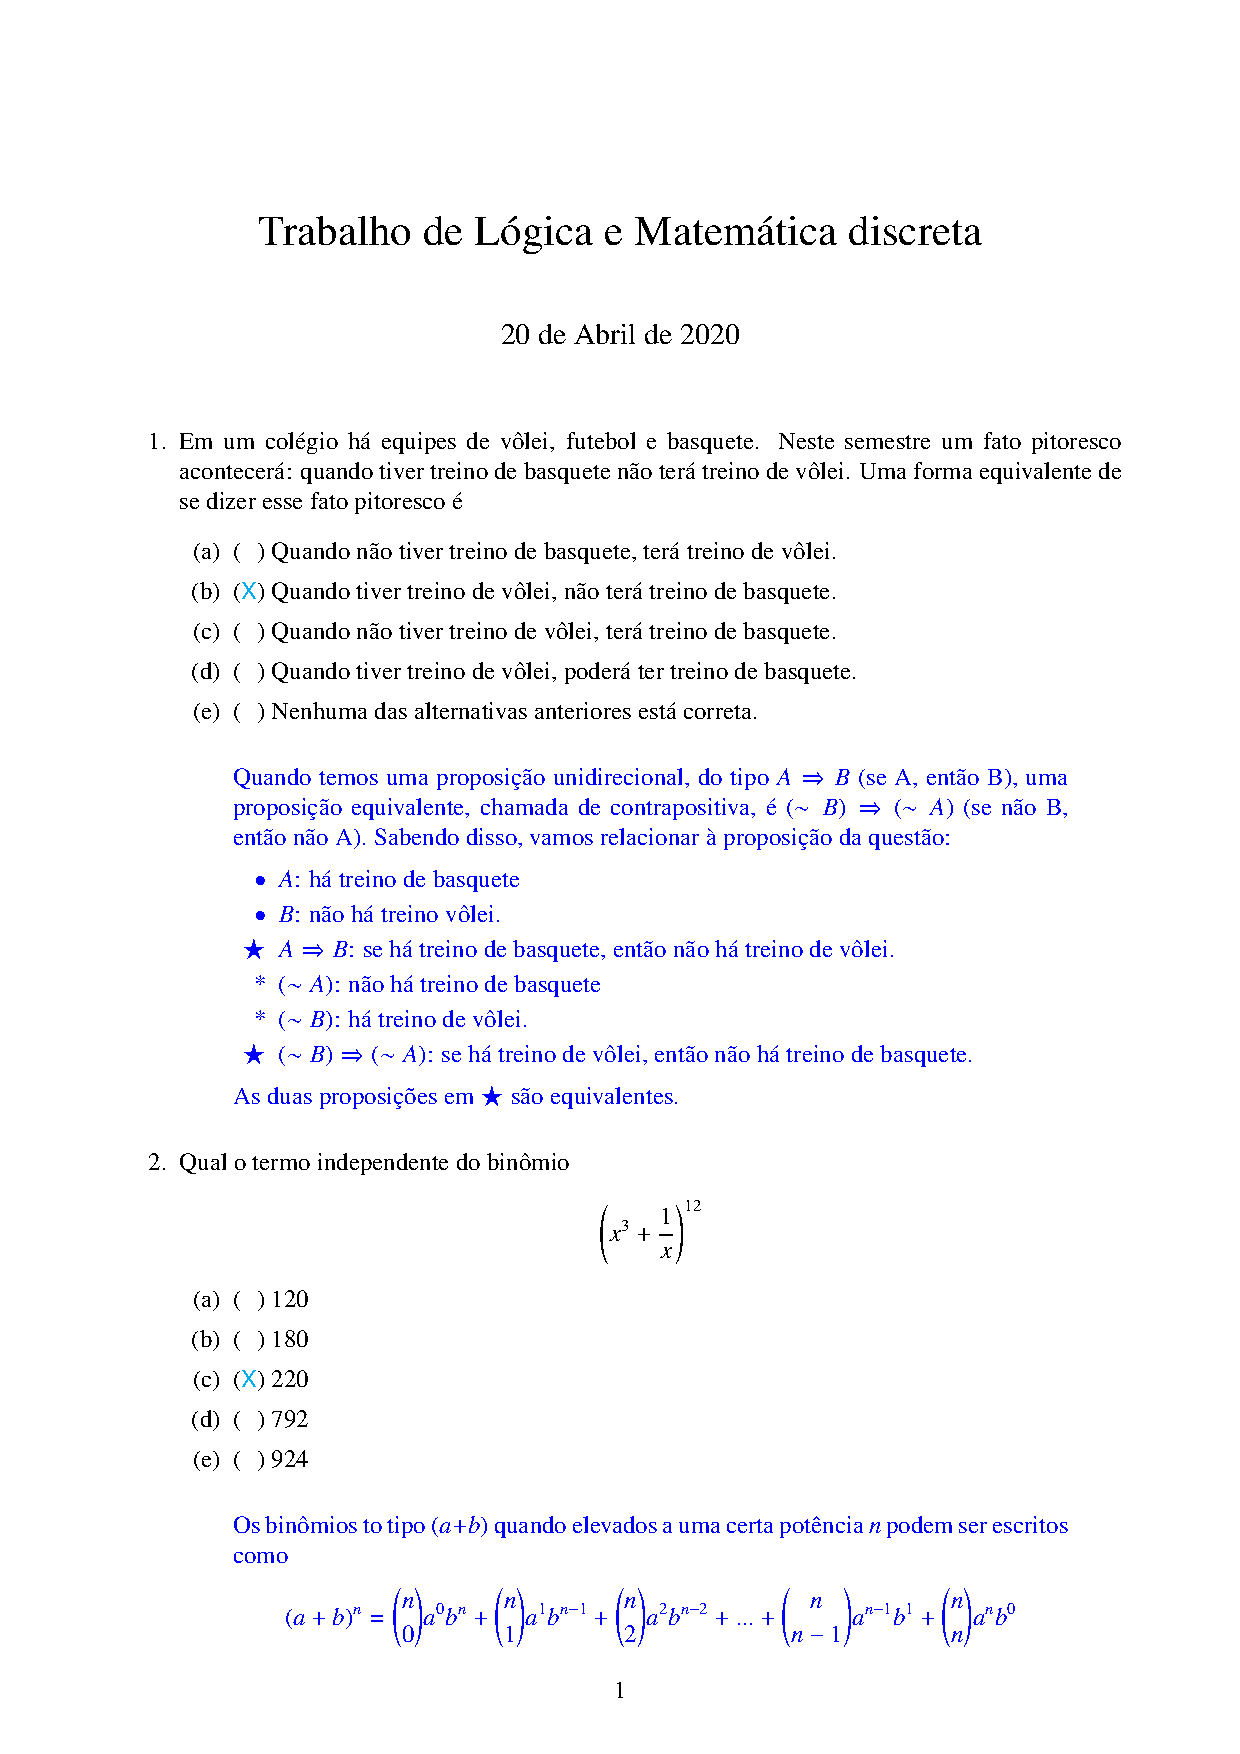
\includepdf[pages=-]{md}






\end{document}

